\subsection{Koppelgetriebe \hfill IP}
\begin{footnotesize}
    \begin{itemize}
        \item Kleinstes Glied der Viergelenkkette ist voll drehfähig, wenn:
        \begin{empheq}[box=\fbox]{align*}
            \text{Glied}_{\text{min}} + \text{Glied}_{\text{max}} < \text{Glied}_{\text{Rest1}} + \text{Glied}_{\text{Rest2}}
        \end{empheq}
        \item \textbf{drehfähig} $\Rightarrow$ laufsicher
        \item \textbf{nicht drehfähig} $\Rightarrow$ durchschlagend
    \end{itemize}
    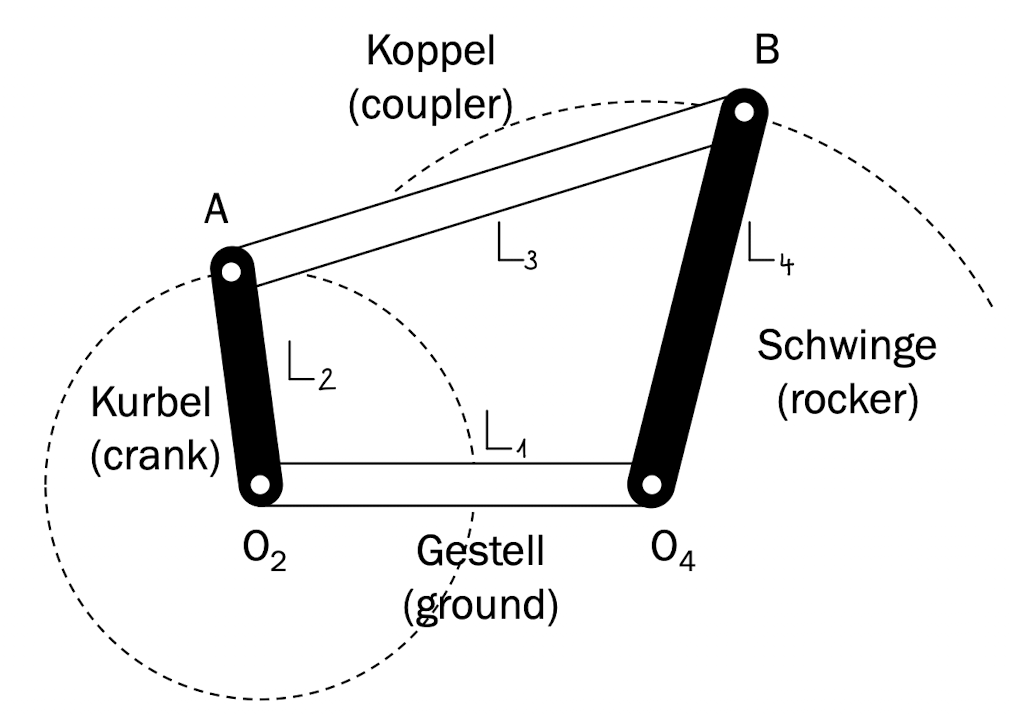
\includegraphics[width = 0.4\linewidth]{src/images/MAEIP_Viergelenkkette}
\end{footnotesize}

\subsubsection{Lambda-Mechanismus \hfill IP}
\begin{footnotesize}
    \begin{minipage}{0.4\linewidth}
        \begin{center}
            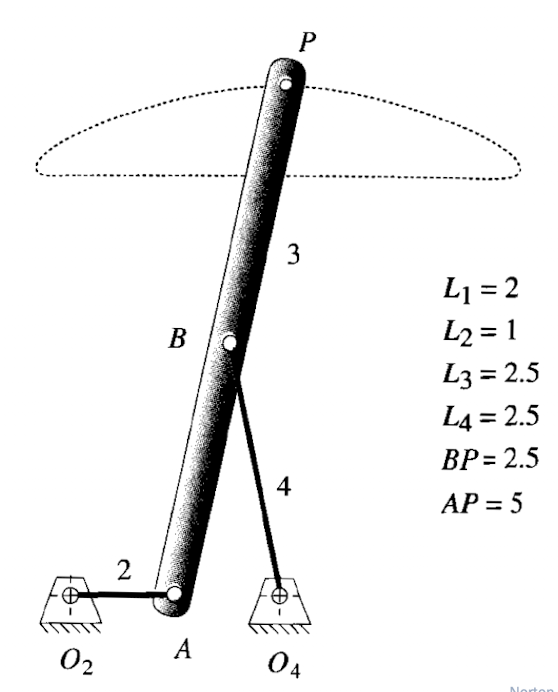
\includegraphics[width = 0.8\linewidth]{src/images/MAEIP_LambdaMechanismus}
        \end{center}    
    \end{minipage}
    \begin{minipage}{0.58\linewidth}
        \begin{center}
            links: Single-Straight-Kurve
            \begin{empheq}[box=\fbox]{align*}
                &\text{fast gerade Linie bei fast} 
                \\ & \text{konstanter Geschwindigkeit}
                \\ &AP \approx 5\cdot L_2 \quad \mid \quad \gamma = 180^\circ
                \\ & \Rightarrow \text{grosser Bauraum}
            \end{empheq}
        \end{center}
    \end{minipage}
\end{footnotesize}